\subsection{MetaClust}
By clicking on the Toolset tab and then choose MetaClust,
users are directed to MetaClust home page as in Figure~\ref{fig:metaClustHome}.
MetaClust \citep{huo2016meta} aims to perform sample clustering analysis combining multiple transcriptomic studies.
By integrating information from multiple studies of similar biological purposes,
MetaClust can identify an unified intrinsic gene set among all studies, perform weighted clustering analysis using the common intrinsic gene set and
match the clustering patterns across studies to define disease subtypes/cluster types.
The resulting clustering from meta-analysis is more robust and accurate than single study analysis.
The R package for MetaClust module can be found at \url{https://github.com/metaOmics/MetaSparseKmeans}.


\begin{figure}[H]
\begin{center}
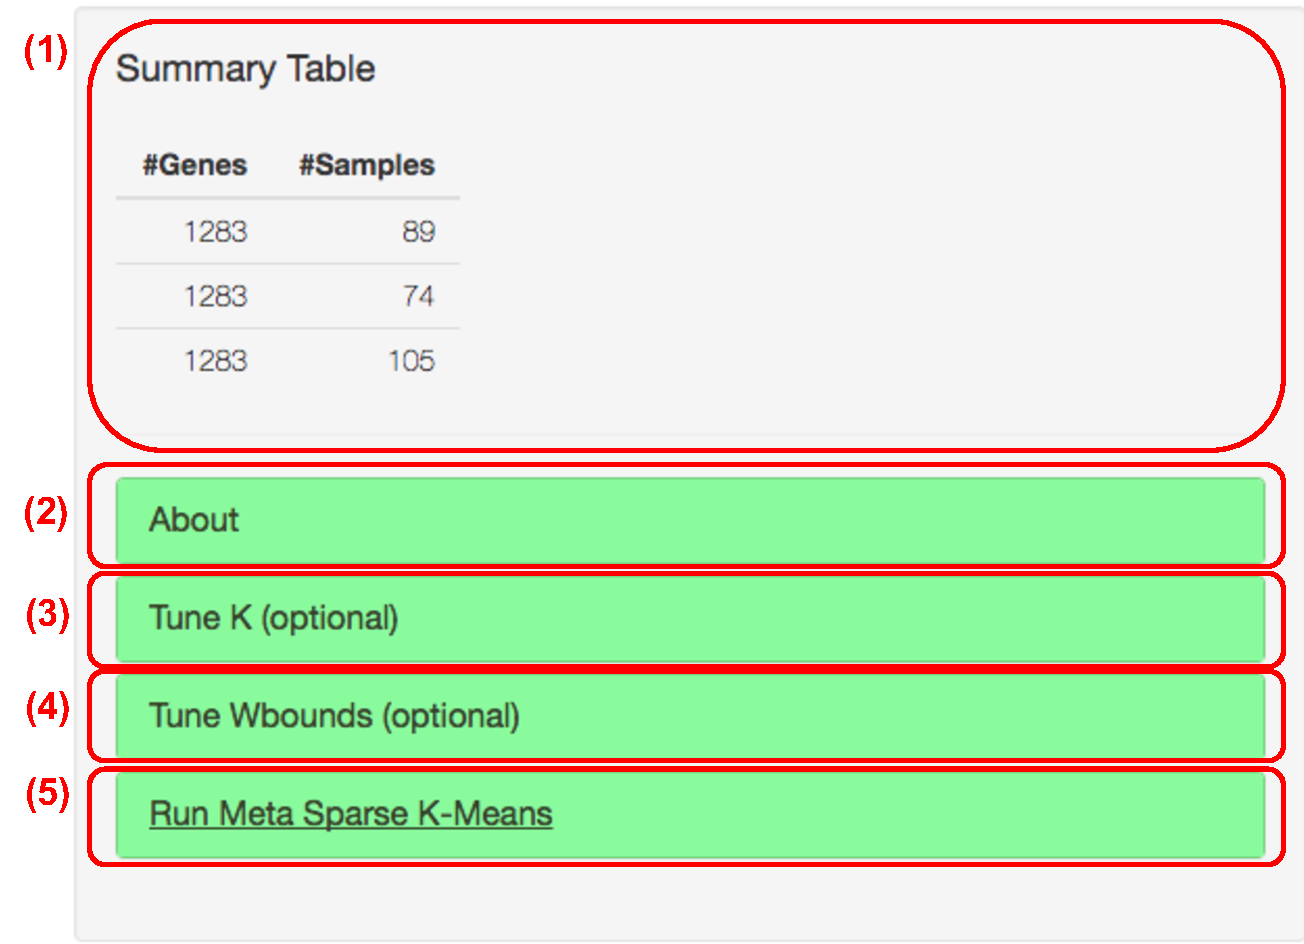
\includegraphics[scale=0.4]{./figure/metaClust/metaClustHome.pdf}
\caption{MetaClust home page}
\label{fig:metaClustHome}
\end{center}
\end{figure}

\subsubsection{Procedure}


Figure~\ref{fig:metaClustHome} shows the home page of MetaClust.
On the top left panel users can see the data summary Table {\color{red} (1)}.
Below there are four tabs. 
About tab {\color{red} (2)} which includes basic introduction of MetaClust, Two tabs for Tune K as well as Wbounds, and the Run Meta Sparse $K$-Means tab.
Starting with multiple studies, 
we could run MetaSparseKmeans {\color{red} (5)} with pre-specified number of clusters ($K$) and gene selection tuning parameter (Wbounds).
If you are not sure about what are good $K$ and Wbounds, please try Tune $K$ {\color{red} (3)} and Tune Wbounds {\color{red} (4)} panel.
A complete list of options is available in Section~\ref{sec:completeList_MetaClust}.

\begin{steps}

\item \textbf{Tune $K$:} 

\begin{figure}[H]
\begin{center}
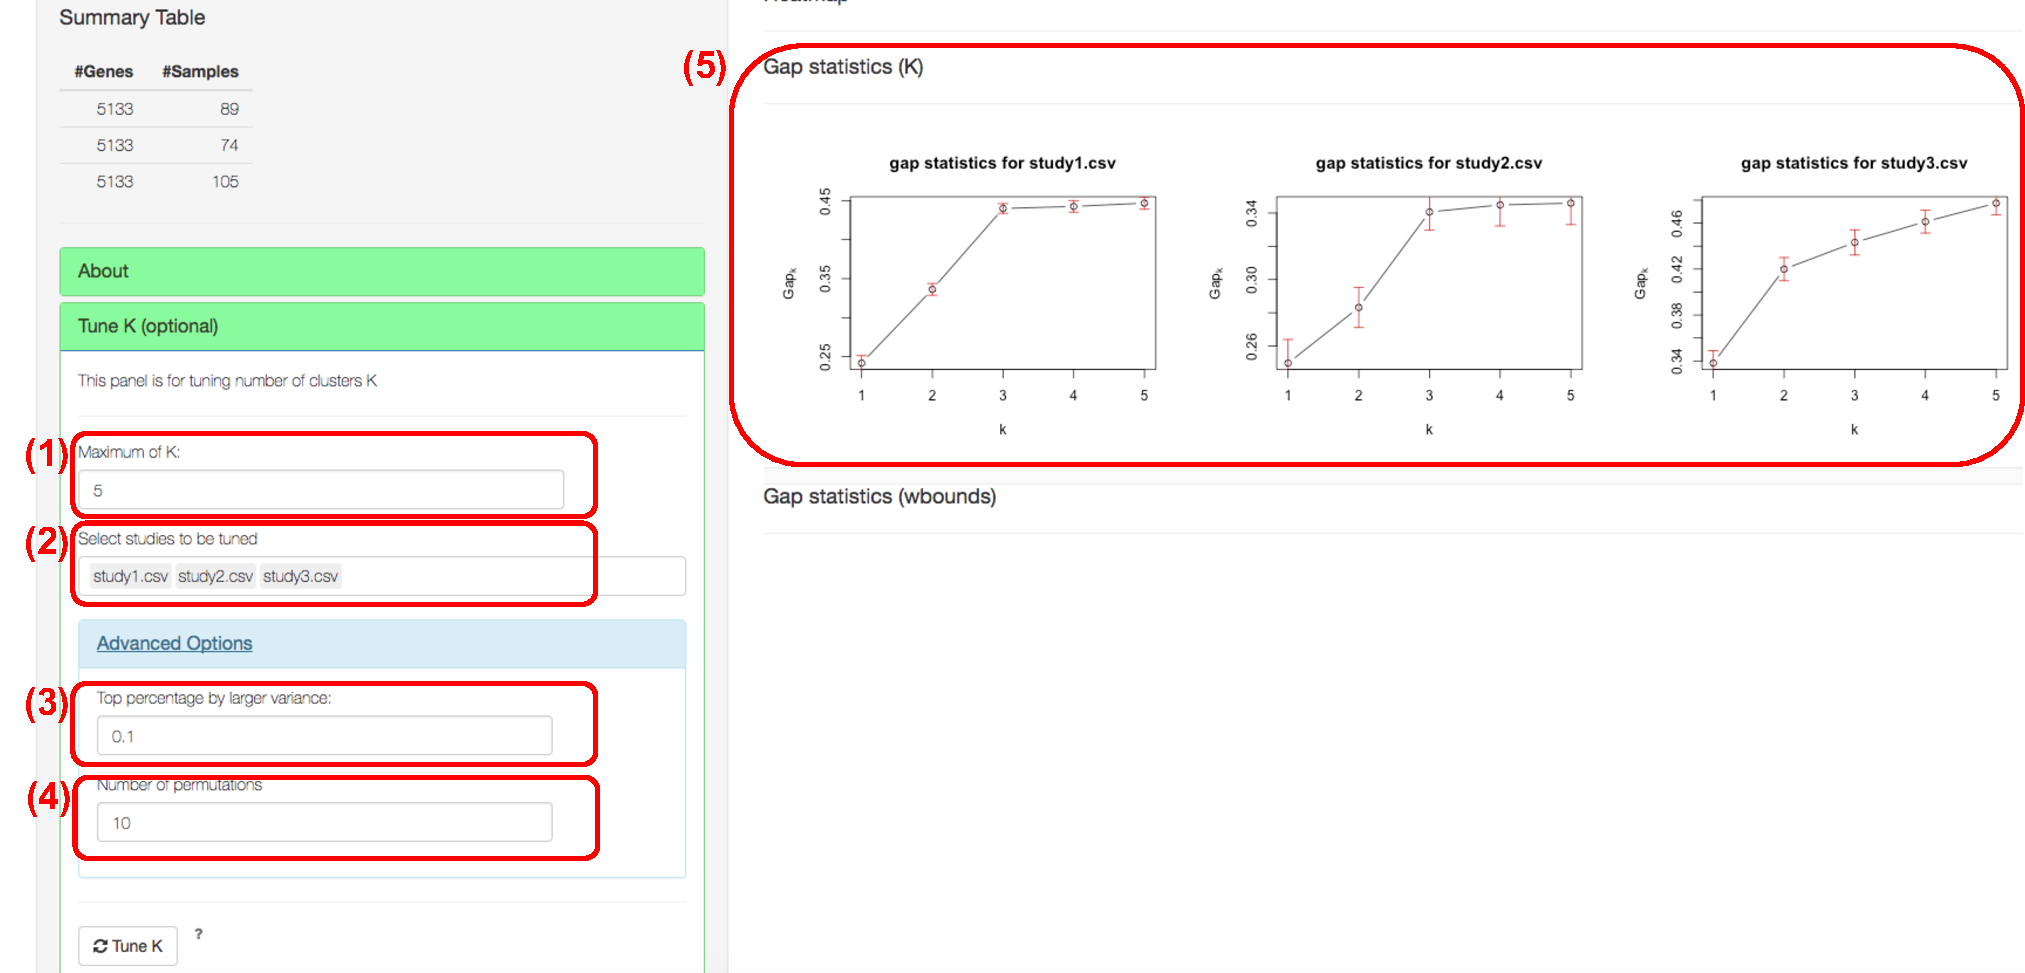
\includegraphics[scale=0.5]{./figure/metaClust/tuneK.pdf}
\caption{Tuning parameter selection for number of clusters.
A good $K$ is selected such that the $\mbox{Gap}_k$ is maximized or stabilized across all studies.
}
\label{fig:metaClusttuneK}
\end{center}
\end{figure}

If the users are not sure what is the number of clusters,
they can start to use the Tune $K$ panel as in Figure~\ref{fig:metaClusttuneK}.
Gap statistics will be used to get optimal $K$ for each individual study.
Detailed description about Gap statistics can be found \cite{tibshirani2001estimating}.
Users need to specify maximum number of $K$ {\color{red} (1)}, which the algorithm will search number of studies from 1 to $K$.
Studies to be tuned can be selected {\color{red} (4)}.
In advanced options, users can further specify number of top variance genes to be included and number of permutations.
But if users don't know the algorithm, please leave them as default.
Top percentage p\% by larger variance means that we will use top p\% larger variance genes to perform gap statistics {\color{red} (3)}.
Number of permutation is the number of bootstrap samples for gap statistics {\color{red} (4)}.
At least 50 bootstrap samples are suggested for a stable result of number of clusters.
By clicking button ``Tune $K$",
we will obtain gap statistics as in Figure~\ref{fig:metaClusttuneK}.
A good $K$ is selected such that the $\mbox{Gap}_k$ is maximized or stabilized across all studies.
From the figure, $K=3$ is preferred since the gap statistics from all three studies become flat {\color{red} (5)}.

\item \textbf{Tune Wbounds:} 

Wbounds directly control number of features selected by metaClust.
A larger number of Wbounds will result in more number of selected genes.
If the users are not sure what is a good Wbound,
they can start to use the Tune Wbounds panel as in Figure~\ref{fig:metaClusttuneW}.
\begin{figure}[H]
\begin{center}
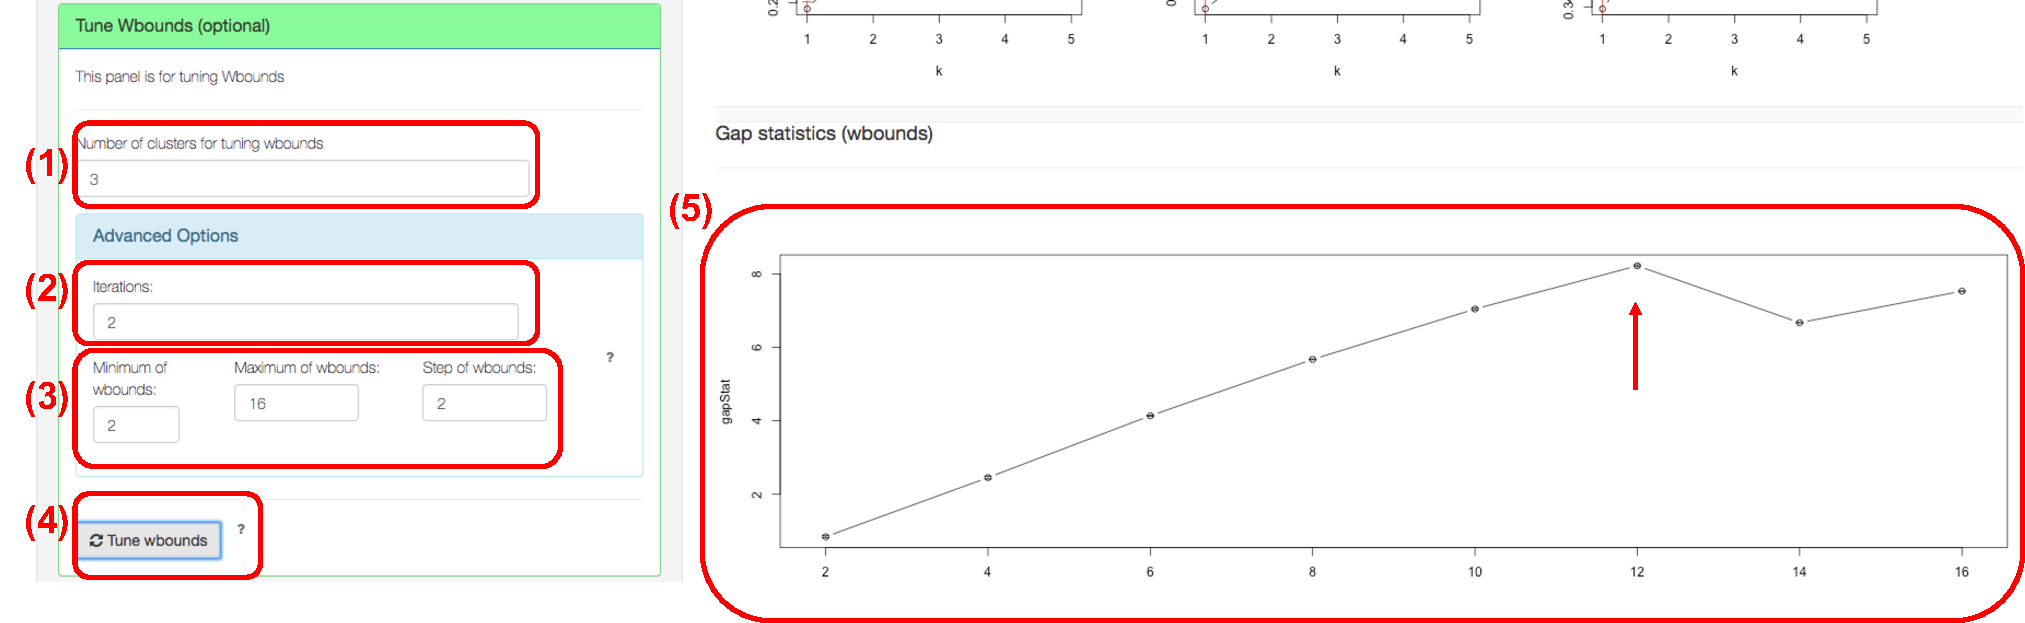
\includegraphics[scale=0.5]{./figure/metaClust/tuneW.pdf}
\caption{Wbound selection.
The Wbound controls the number of selected features.
A larger Wbound will yield a larger number of selected genes.
The optimum Wbound is selected when the gap statistics is maximized.
}
\label{fig:metaClusttuneW}
\end{center}
\end{figure}
Again,
gap statistics will be used for tuning Wbounds.
Users will specify number of clusters for tuning Wbounds {\color{red} (1)}, which could be obtained from the previous step.
In advanced options, users can further specify the number of iterations and the range of candidate Wbounds.
But if users don't know the algorithm, please leave them as default.
Iterations {\color{red} (2)} specify number of bootstrap samples for gap statistics.
Users also need to specify the searching space of Wbounds by minimum of Wbounds, maximum of Wbounds and Step of Wbounds {\color{red} (3)}.
After all these steps are set,
user can click on ``Tune Wbounds" button {\color{red} (4)}.
The results will be shown in Figure~\ref{fig:metaClusttuneW} {\color{red} (5)}.
Wbound=12 is preferred since the corresponding gap statistics is maximized (where the red arrow indicates).

\item \textbf{Run MetaClust:} 

Under Run Meta Sparse K-Means panel,
user can specify the number of clusters {\color{red} (1)}, Wbounds {\color{red} (2)} and run MetaClust {\color{red} (5)} 
as in Figure~\ref{fig:mskmRes}.
\begin{figure}[H]
\begin{center}
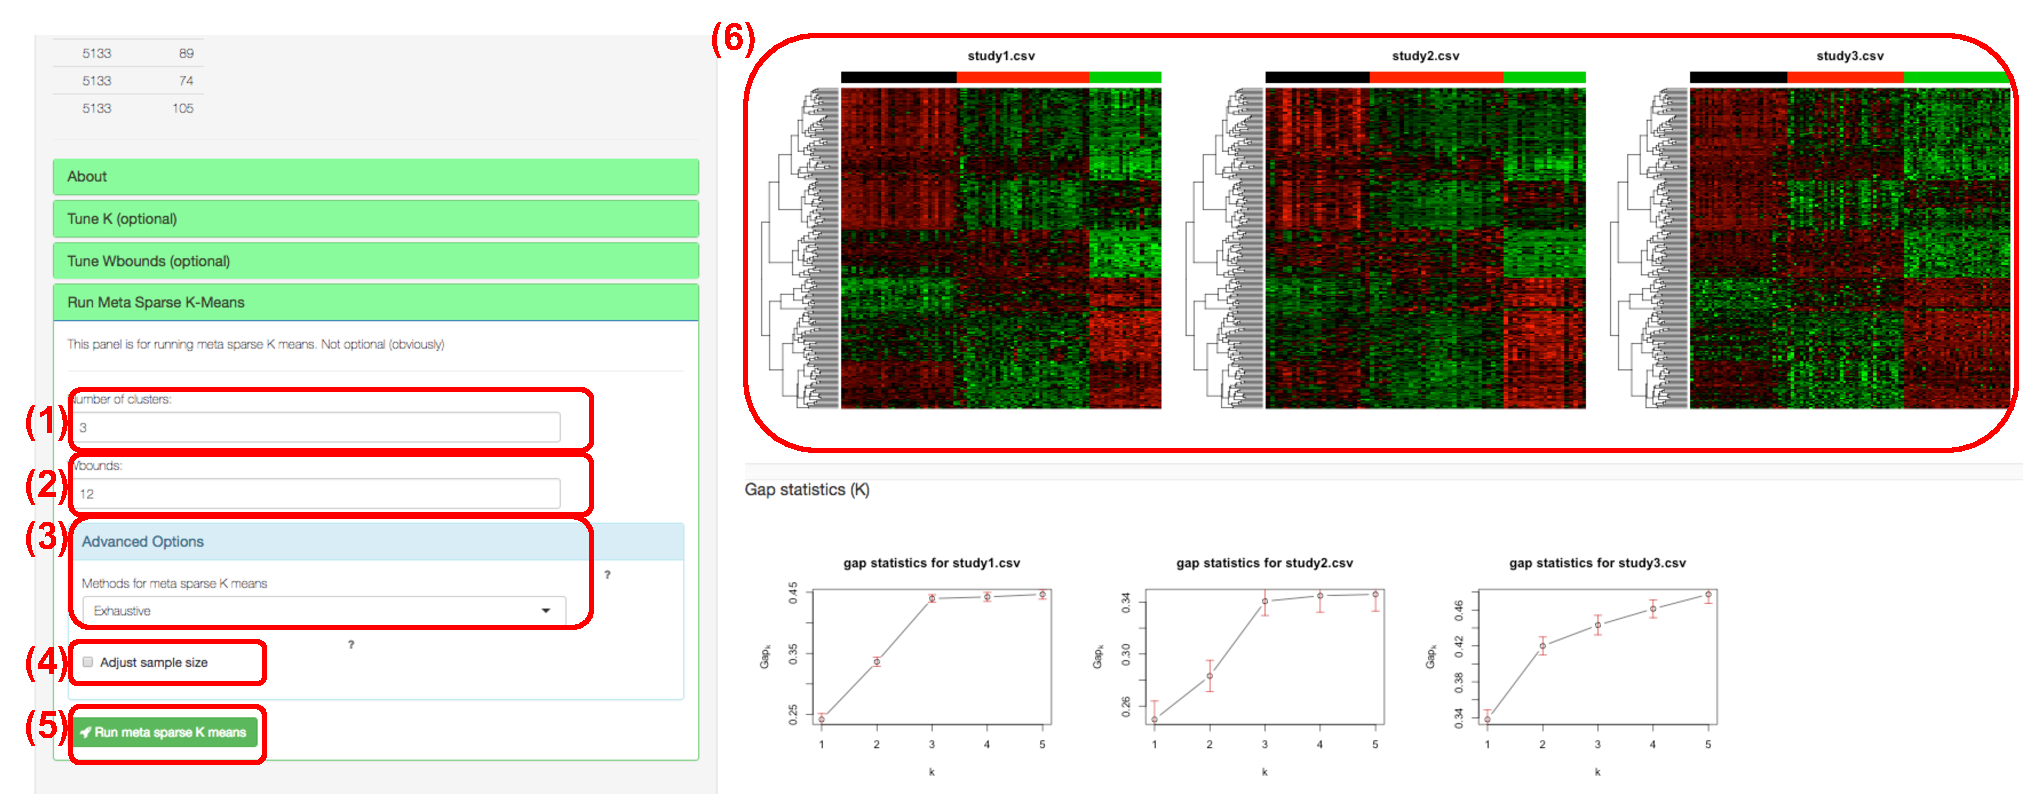
\includegraphics[scale=0.5]{./figure/metaClust/mskmRes.pdf}
\caption{Result for MetaClust.
The heatmap on top show the gene expression profiles of the three studies with selected features.
Each row represents a gene and each column represents a sample.
Note that the three studies share a common set of genes.
The color bar on top of the heatmap represent the subtype labels.
For instance, the black bar on top of each studies represents subtype one for all studies.
Clearly, we could see distinct subtype patterns and these patterns are consistent across studies.
}
\label{fig:mskmRes}
\end{center}
\end{figure}
In advanced options (for which users are not suggested to change if they are not familiar with the algorithm), 
There are three clustering matching methods {\color{red} (3)}: Exhaustive, linear, MCMC.
Exhaustive is suggested if the data is not large.
Currently, only Exhaustive search method is implemented.
Adjust sample size checkbox (at position {\color{red} (5)}) allows users to adjust sample size effect.
After number of clusters and Wbounds are specified,
users can click on Run meta sparse $K$ means and obtain results as Figure~\ref{fig:mskmRes}.
\end{steps}


\subsubsection{Results}

We used the leukemia data to demonstrate the MetaClust module.
After merging the three datasets, we didn't filter out any genes (filter 0\% genes by mean and 0\% by variance) thus 5133 genes remained.
Detailed descriptions of these studies can be found in Table~\ref{tab:realDataLeukemia}. 
In this example, we do not need the extra label information.
The result is shown in Figure~\ref{fig:mskmRes} {\color{red} (5)}.
We obtained unified feature selection across all studies.
The clusters are well separated in each study and the cluster patterns are consistent across all studies.
The clustering heatmaps and labels are saved in the MetaClust folder.










